\section{2005 - PHYSICS 2A ALTERNATIVE A PRACTICAL}

\begin{enumerate}
\item[1.] The aim of this experiment is to determine the mass of unknown weight labelled \textbf{X} and the force constant of the spring \textbf{k}.

\begin{center}
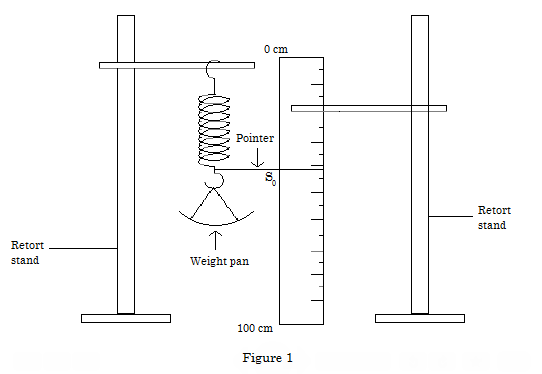
\includegraphics[width=12cm]{./img/2005-1-alt.png}
\end{center}

Set up the apparatus provided as shown in figure 1 above. Add 50 g mass on to the weight pan so that any ``kinks'' in the spring are removed. Leave this weight for the whole experiment but ignore it in all readings. Record the scale reading $S_0$. Add 50 g on to the weight pan and record the new scale reading $S$. Calculate the extension ($e = S - S_0$) caused by the weight. Repeat with different weights ($W$) to obtain at least five readings. Tabulate your results. Replace the weights ($W$) by the weight \textbf{X} provided and find the corresponding extension.\\[10pt]

Record this extension as $S_{\text{X}}$ ............. cm

\begin{enumerate}
\item[(a)] Plot a graph of load against extension.
\item[(b)]
\begin{enumerate}
\item[(i)] Find the gradient (G) of your graph.
\item[(ii)] What is the physical meaning of the gradient?
\end{enumerate}
\item[(c)] From the graph, what is the mass of the weight labelled \textbf{X}?
\end{enumerate}

\item[2.] The aim of this experiment is to find the critical angle \textbf{C} of the given glass block.

\begin{center}
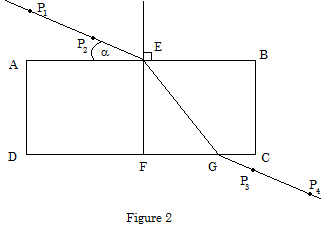
\includegraphics[width=10cm]{./img/2005-2-alt.png}
\end{center}

\textbf{Proceed as follows:}\\[10pt]

Place a white sheet of paper on the drawing board. Place the glass block, with one of its largest surfaces top most on top of the white paper. Mark the outline of the glass block on the paper with a pencil. Then remove the glass block and draw a line which cuts its largest sides normally at E and F as shown in figure 2 above. \\[10pt]

Using a protractor draw an angle $\alpha = 30^\circ$ with the glass block. Replace the glass block in its original position and stick the first pin P$_1$ and second pin P$_2$ along the line of angle $\alpha = 30^\circ$. Stick the third and fourth pins P$_3$ and P$_4$ respectively on the opposite side of the glass block such that P$_3$ and P$_4$ fall on a straight line with P$_1$ and P$_2$ when viewed through side CD of the glass block. \\[10pt]

Remove the glass block and trace the straight path taken by the ray G P$_3$ P$_4$. Using a ruler, join G and E. \\[10pt]

Measure the angle of refraction $r^\circ$, then calculate the values of $\cos{\alpha}$ and $\sin{r^\circ}$. Repeat the same procedure for values $\alpha = 40^\circ$, $50^\circ$, $60^\circ$, $70^\circ$ and $80^\circ$. Record your results in tabular form for the values of $\alpha$, $r^\circ$, $\sin{r^\circ}$ and $\cos{\alpha}$.

\begin{enumerate}
\item[(a)] Plot a graph of $\sin{r^\circ}$ (vertical axis) against $\cos{\alpha}$ (horizontal axis).
\item[(b)] Find the slope of the graph.
\item[(c)] Calculate the value of $C$ where slope = $\sin{C}$.
\item[(d)] State the possible sources of error and precautions you have taken during the experiment.
\end{enumerate}

\item[3.] The aim of this experiment is to determine the \textbf{e.m.f. E} and internal resistance \textbf{r} of a cell.

\begin{center}
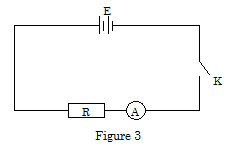
\includegraphics[width=7cm]{./img/2005-3-alt.png}
\end{center}

\begin{enumerate}
\item[(a)] Connect the circuit as shown in figure 3 above. Put $R = 1 \Omega$ and quickly read the value of $i$ on the ammeter.
\item[(b)] Repeat the procedure in 3 (a) above, for values of $R = 2 \Omega$, $3 \Omega$, $4 \Omega$ and $5 \Omega$ respectively.
\item[(c)] Tabulate your results and complete the following table.
\begin{center}
\begin{tabular}{|c|c|c|} \hline
\textbf{Resistance $R$ ($\Omega$)} & \textbf{Current $i$ (A)} & \textbf{$\cfrac{1}{i} \left(\text{A}^{-1}\right)$ } \\ \hline
1&& \\
2&& \\
3&& \\
4&& \\
5&& \\ \hline
\end{tabular} \\[10pt]
\end{center}
\item[(d)] Plot the graph of $R$ against $\cfrac{1}{i}$.
\item[(e)] The graph uses the equation $R = \cfrac{E}{i} - r$.
\begin{enumerate}
\item[(i)] Suggest how $E$ and $r$ may be evaluated from your graph.
\item[(ii)] Evaluate $E$ for one cell.
\item[(iii)] Evaluate $r$ for one cell.
\end{enumerate}
\item[(f)] State one source of error and suggest one way of minimizing it.
\end{enumerate}

\end{enumerate}